% Figure: the complexity landscape at a glance.
% Requires only tikz. Colors are Okabe--Ito tints (colorblind-safe); every cell also states its bound in text.
\begin{figure}[t]
\centering
\providecommand\Description[2][]{}%
\Description{A four-by-four grid. Rows: beta zero, beta one, beta two, beta p for p at least three. Columns: the universe is a graph, a complex in three-space, a two-complex in four-space, or arbitrary. Green cells (polylogarithmic) fill the beta-zero row, the beta-one cell of the graph column, and the beta-one and beta-two cells of the three-space column; orange cells (hard under OMv) fill beta one and beta two in four-space and all higher rows for arbitrary complexes; gray cells are identically zero. A dashed line separates the three-space and four-space columns.}
\definecolor{lsEasy}{HTML}{009E73}%
\definecolor{lsHard}{HTML}{D55E00}%
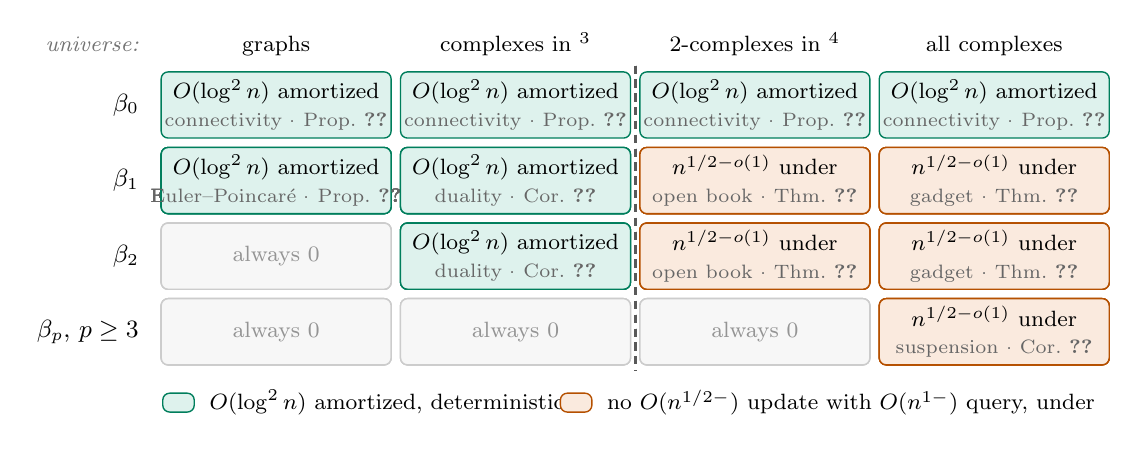
\begin{tikzpicture}[x=1cm,y=1cm,font=\footnotesize,
  cellbox/.style={rounded corners=2.5pt,line width=0.5pt},
  easy/.style={cellbox,fill=lsEasy!13,draw=lsEasy!80!black},
  hard/.style={cellbox,fill=lsHard!13,draw=lsHard!85!black},
  zero/.style={cellbox,fill=black!3,draw=black!20},
  hdr/.style={align=center,inner sep=1pt}]
  \def\cw{3.04}\def\ch{0.96}\def\gp{0.06}\def\xo{1.3}
  % \lscell{column}{row}{style}{bound}{method}{reference}
  \def\lscell#1#2#3#4#5#6{%
    \path[#3] ({\xo+#1*\cw+\gp},{-#2*\ch-\gp}) rectangle ({\xo+(#1+1)*\cw-\gp},{-(#2+1)*\ch+\gp});
    \node[align=center,inner sep=0pt] at ({\xo+(#1+0.5)*\cw},{-(#2+0.5)*\ch})
      {#4\\[0.6pt]{\scriptsize\color{black!60}#5\ \textperiodcentered\ #6}};}
  \def\lszero#1#2{%
    \path[zero] ({\xo+#1*\cw+\gp},{-#2*\ch-\gp}) rectangle ({\xo+(#1+1)*\cw-\gp},{-(#2+1)*\ch+\gp});
    \node[text=black!42] at ({\xo+(#1+0.5)*\cw},{-(#2+0.5)*\ch}) {always $0$};}
  % column headers: the class of the universe
  \foreach \c/\t in {0/{graphs},1/{complexes in $\R^3$},2/{$2$-complexes in $\R^4$},3/{all complexes}}
    \node[hdr,anchor=base] at ({\xo+(\c+0.5)*\cw},0.2) {\t};
  \node[anchor=base east,text=black!55,font=\footnotesize\itshape] at ({\xo-0.1},0.2) {universe:};
  % row headers
  \foreach \r/\t in {0/{$\beta_0$},1/{$\beta_1$},2/{$\beta_2$},3/{$\beta_{p}$, $p\ge3$}}
    \node[anchor=east] at ({\xo-0.1},{-(\r+0.5)*\ch}) {\small\t};
  % beta_0: dynamic connectivity, in every universe
  \foreach \c in {0,1,2,3} \lscell{\c}{0}{easy}{$O(\log^2 n)$ amortized}{connectivity}{Prop.~\ref{prop:beta0}}
  % beta_1
  \lscell{0}{1}{easy}{$O(\log^2 n)$ amortized}{Euler--Poincar\'e}{Prop.~\ref{prop:beta0}}
  \lscell{1}{1}{easy}{$O(\log^2 n)$ amortized}{duality}{Cor.~\ref{cor:anyR3}}
  \lscell{2}{1}{hard}{$n^{1/2-o(1)}$ under \OMv}{open book}{Thm.~\ref{thm:r4}}
  \lscell{3}{1}{hard}{$n^{1/2-o(1)}$ under \OMv}{gadget}{Thm.~\ref{thm:omv}}
  % beta_2
  \lszero{0}{2}
  \lscell{1}{2}{easy}{$O(\log^2 n)$ amortized}{duality}{Cor.~\ref{cor:anyR3}}
  \lscell{2}{2}{hard}{$n^{1/2-o(1)}$ under \OMv}{open book}{Thm.~\ref{thm:r4}}
  \lscell{3}{2}{hard}{$n^{1/2-o(1)}$ under \OMv}{gadget}{Thm.~\ref{thm:omv}}
  % beta_p, p >= 3
  \lszero{0}{3}
  \lszero{1}{3}
  \lszero{2}{3}
  \lscell{3}{3}{hard}{$n^{1/2-o(1)}$ under \OMv}{suspension}{Cor.~\ref{cor:allp}}
  % the dimension dichotomy between R^3 and R^4
  \draw[line width=1pt,black!65,dash pattern=on 3pt off 2pt] ({\xo+2*\cw},0.02) -- ({\xo+2*\cw},{-4*\ch-0.02});
  % legend, centred under the grid
  \begin{scope}[shift={({\xo+2*\cw},{-4*\ch-0.42})}]
    \path[easy] (-6.0,-0.12) rectangle (-5.6,0.12);
    \node[anchor=west] at (-5.53,0) {$O(\log^2 n)$ amortized, deterministic};
    \path[hard] (-0.95,-0.12) rectangle (-0.55,0.12);
    \node[anchor=west] at (-0.48,0) {no $O(n^{1/2-\eps})$ update with $O(n^{1-\eps})$ query, under \OMv};
  \end{scope}
\end{tikzpicture}
\caption{Maintaining one Betti number of a subcomplex~$K$ of a fixed universe with $n$ simplices under single-simplex insertions and deletions; the columns give the class of the universe.
Green: deterministic data structures with $O(\log^2 n)$ amortized update time and constant query time, after polynomial preprocessing.
Orange: assuming the \OMv\ conjecture, for every $\eps>0$ and over every field, no data structure with polynomial preprocessing time has amortized update time $O(n^{1/2-\eps})$ and query time $O(n^{1-\eps})$; over~$\Ftwo$, each of these problems is equivalent, up to constant factors, to dynamic matrix rank (Corollary~\ref{cor:equiv}, and Corollary~\ref{cor:r4-equiv} for~$\R^4$), and over every field the problems in the last column are equivalent to dynamic rank of $\{0,\pm1\}$-matrices.
The second line of a cell names the method: the \emph{gadget} of Section~\ref{sec:equiv}; the \emph{open book}, an explicit linear form of the embedding of Edelsbrunner and Parsa~\cite{EP14} applied to the gadget (Section~\ref{sec:lower-r4}); \emph{suspension}, which shifts Betti numbers up by one dimension (Lemma~\ref{lem:suspension}); and Alexander \emph{duality} (Section~\ref{sec:easy-s3}).
The dashed line marks the dichotomy between three and four dimensions; Table~\ref{tab:landscape} gives the precise bounds and further settings.}
\label{fig:landscape}
\end{figure}
